\subsection{Colors > Set Unique}
\label{subsection:setUniqueColor}

\begin{figure}[!htb]
\begin{center}
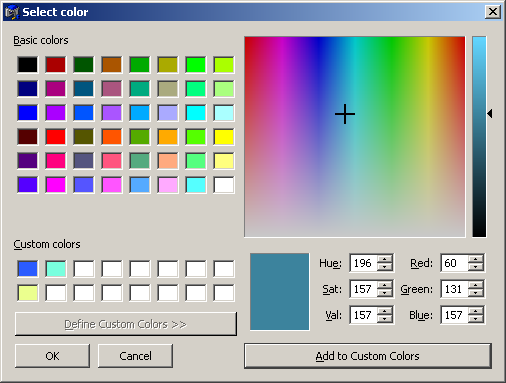
\includegraphics[width=0.5\textwidth]{Partie3_Fonctions/colorSelectionDlg.png}
\caption{\label{fig:colorSelectionDlg}Interface de s�lection d'une couleur unique}
\end{center}
\end{figure}

\index{couleurs}
Permet de d�finir une couleur qui sera appliqu�e � tous les points/sommets des entit�s 3D s�lectionn�es. 
Le choix est manuel, et se fait via une interface classique proposant divers modes de s�lection (figure~\ref{fig:colorSelectionDlg}) :
\begin{itemize}
\item soit en choisissant une couleur \emph{basique} (en haut � gauche),
ou une couleur pr�c�demment sauvegard�e (\emph{custom} - en bas � gauche)
\item soit en cliquant sur la zone color�e (en haut � droite) et en faisant varier l'intensit� avec l'ascenseur
en d�grad� (� droite)
\item soit en rentrant manuellement les param�tres dans les trois champs HSV ou RGB (en bas � droite)
\end{itemize}
\par
Raccourci clavier : \textcolor{red}{ALT+C}

